\subsection{Builder}
\label{builder}

\textbf{Scopo}: Creazionale \\
\textbf{Raggio d'azione}: Oggetti

\paragraph{Definizione} Il patter Builder permette di separare la costruzione di un oggetto complesso dalla sua rappresentazione, in modo che lo stesso processo di costruzione possa essere utilizzato per creare rappresentazioni diverse.

\paragraph{Problema} Prendiamo in considerazione un’applicazione capace di leggere documenti in formato RTF che può supportare la conversione in altri formati (ASCII, LaTeX).

\begin{figure}[H]
    \centering
    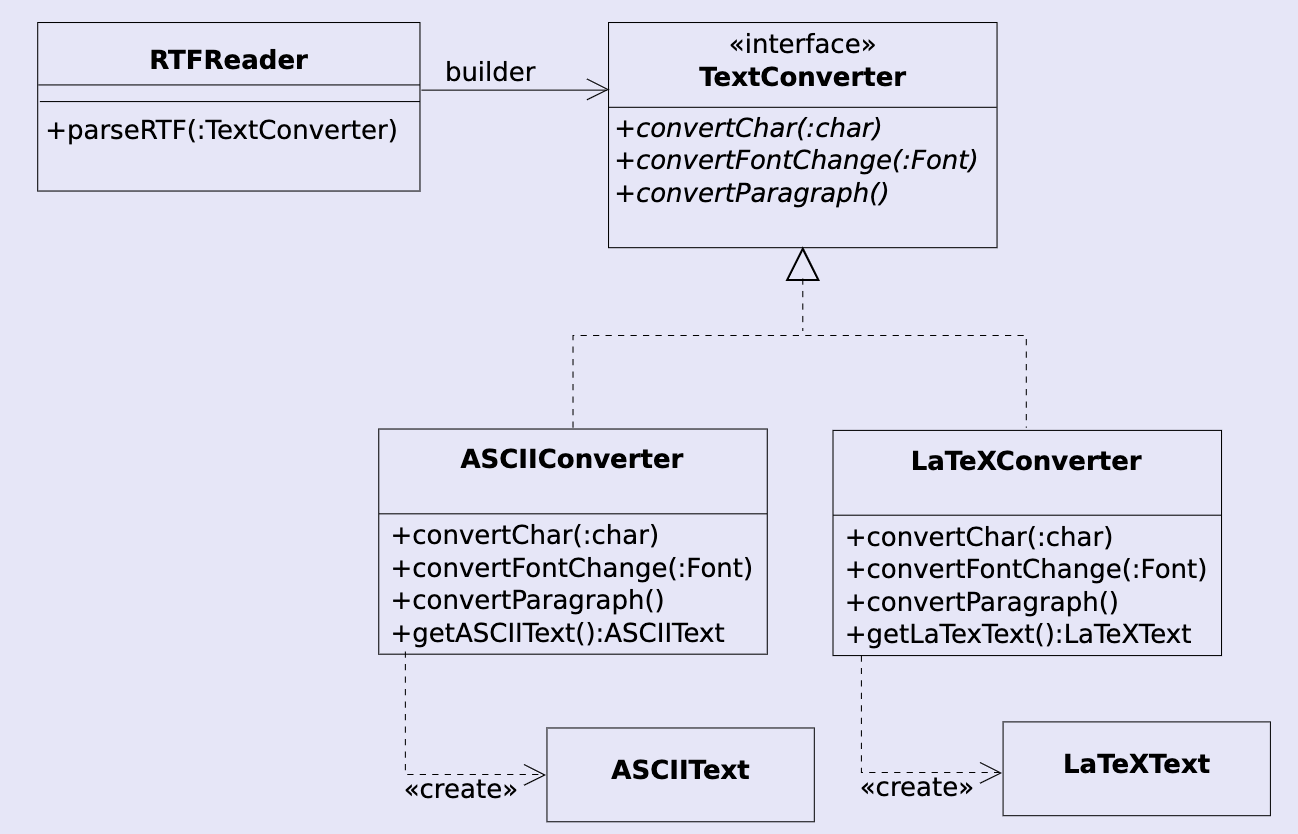
\includegraphics[width=1\linewidth]{assets/pattern/builder/builder-esempio.png}
\end{figure}

\paragraph{Soluzione} Una soluzione consiste nel configurare la classe RTFReader con un oggetto conforme all’interfaccia TextConverter in grado di gestire la conversione in un altro formato. Il documento nel formato di uscita viene costruito man mano che gli elementi del documento RTF sono analizzati.

\begin{figure}[H]
    \centering
    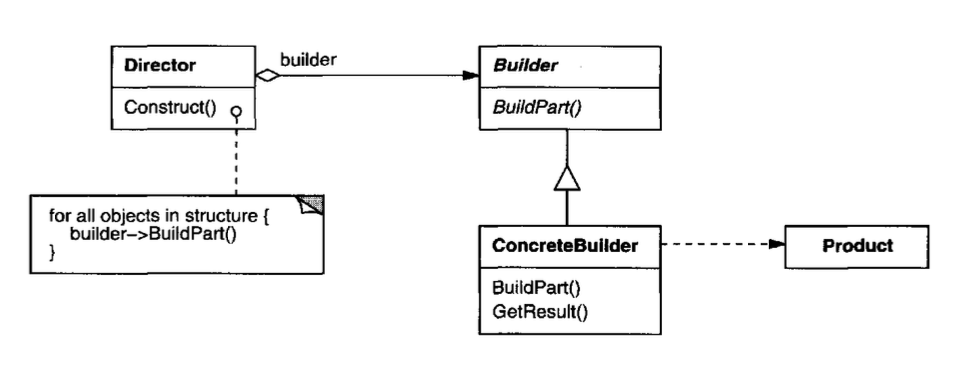
\includegraphics[width=1\linewidth]{assets/pattern/builder/builder-struttura.png}
\end{figure}

\paragraph{Struttura e Conseguenze} Il pattern è composto da:
\begin{itemize}
    \item \textbf{BuilderIF}: specifica l’interfaccia astratta che crea le parti dell’oggetto Product. 
    \item \textbf{ConcreteBuilder}: costruisce e assembla le parti del prodotto implementando l’interfaccia Builder; definisce e tiene traccia della rappresentazione che crea.
    \item \textbf{Director}: costruisce un oggetto utilizzando l’interfaccia Builder.
    \item \textbf{Product}: rappresenta l’oggetto complesso e include le classi che definiscono le parti che lo compongono, includendo le interfacce per assemblare le parti nel risultato finale.
\end{itemize}

Permette quindi di: variare la rappresentazione interna di un prodotto, isolare il codice per la costruzione la rappresentazione e consente di avere maggiore controllo del processo di costruzione.

Risolve allo stesso tempo il problema dei \textbf{costruttori telescopici}, e si propone come alternativa a tecnologie come JavaBeans.

\newpage

\textbf{Esempio Java}

\begin{minted}[
    fontsize=\footnotesize,
    linenos,
]{java}
public class NutritionFacts { 

    private final int servingSize; 
    private final int servings; 
    private final int calories ; 
    private final int fat ; 
    private final int sodium; 
    private final int carbohydrate; 
    
    public static class Builder { 
        // Required parameters 
        private final int servingSize; 
        private final int servings; 
        
        // Optional 
        private int calories = 0; 
        private int fat = 0; 
        private int carbohydrate = 0; 
        private int sodium = 0; 
        
        public Builder( int servingSize, int servings) { 
            this.servingSize = servingSize; 
            this.servings = servings; 
        } 
        
        public Builder calories ( int val ) { 
            calories = val ; return this;
        } 
        
        public Builder fat ( int val ) { 
            fat = val ; 
            return this; 
        } 
        
        public Builder carbohydrate(int val ) {
            carbohydrate = val; 
            return this; 
        } 
        
        public Builder sodium(int val) { 
            sodium = val; 
            return this; 
        } 
        
        public NutritionFacts build () { 
            return new NutritionFacts(this); 
        } 
    }
    
    private NutritionFacts (Builder builder ) { 
        servingSize = builder.servingSize; 
        servings = builder.servings; 
        calories = builder.calories; 
        fat = builder.fat;
        sodium = builder.sodium; 
        carbohydrate = builder.carbohydrate;
    }
}

// Utilizzo:
NutritionFacts cocaCola = new NutritionFacts.Builder(240, 8)
                            .calories(100)
                            .sodium(35)
                            .carbohydrate(27)
                            .build();

\end{minted}

\paragraph{Interazioni} L'utilizzo del pattern consiste nel creare un oggetto Director e configurarlo tramite l'oggetto Builder. Il Director informa il Builder ogni volta che una parte di Product deve essere costruita. Il Builder riceve e gestisce le richieste dal Director e aggiunge le parti al Product. Il client ottiene dal Builder il Product creato.

\begin{figure}[H]
    \centering
    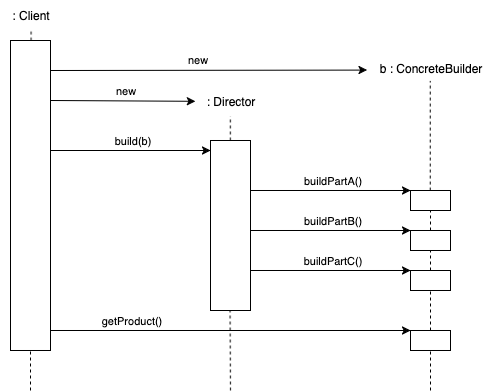
\includegraphics[width=1\linewidth]{assets/pattern/builder/builder-activity.drawio.png}
\end{figure}

\newpage